\documentclass[9pt]{exam}
\usepackage[utf8]{inputenc}		% Caracteres latinos
\usepackage[spanish]{babel}		% Idioma español
\usepackage{geometry}			% Organizar el documento
\usepackage{graphicx}			% Incluir gráficos
\usepackage{makecell}			% Para personalizar las celdas de una tabla
\usepackage[nohdr]{mathexam}	% Añadimos el paquete mathexam (sin header)
\usepackage{amsmath}
\usepackage{amsfonts}
\usepackage{amssymb}
\usepackage{mathtools}
\usepackage{tikz,pgfplots}
\usepgfplotslibrary{polar}
\usepackage[shortlabels]{enumitem}
\usepackage{textpos}
\usepackage{caption}
\usepackage{mwe}
\usepackage{relsize}
 \renewcommand{\baselinestretch}{1.5}
 \usepackage{graphicx}
\newcommand\sbullet[1][.5]{\mathbin{\vcenter{\hbox{\scalebox{#1}{$\bullet$}}}}}
\usepackage{multicol}
%\usepackage[]{mathptmx}        % A free version o Times Roman with mathematical symbols
%\usepackage{pzc}               % fuente cursiva (conjuntos) Zapf Chancery
%\usepackage{showframe}
%\usepackage{lipsum}

% DOCUMENTACIÓN DE LA CLASE EXAM
% http://ftp.inf.utfsm.cl/pub/tex-archive/macros/latex/contrib/exam/examdoc.pdf
% DOCUMENTACIÓN DE LA CLASE MATHEXAM
% http://ctan.dcc.uchile.cl/macros/latex/contrib/mathexam/doc/mathexam.pdf

% Definimos la geometría de la primera página
\geometry{
	a4paper,                    % Tamaño del documento
	hmargin = {1.5cm, 1.5cm}, 	% Margen horizontal izquierdo, derecho
	vmargin = {1.5cm, 1cm},	    % Margen vertical superior, inferior
	headsep = 4mm,				% Separación entre el encabezado y el texto
	head = .2cm,				% Tamaño del encabezado
	% marginparsep = 5mm, 		% Seperación entre las notas y el texto
	% marginpar = 1.5cm,		% Tamaño de las notas
	includeall,                 % incluye el encabezado, footer y notas dentro del tamaño del documento
	nomarginpar,	            % Elimina las notas
	foot = 1cm,                 % Tamaño del footer
	twoside,                	% Habilita el modo de impresión a doble cara
}

\selectlanguage{spanish}        % Selecciona el idioma
\spanishdecimal{.}

%\pagestyle{headandfoot}         % Nuestro examen tendrá encabezado y pié

% DEFINIMOS EL ENCABEZADO
%\header{
%\begin{tabular}{l c c c l}
%            \makecell{\includegraphics[height=2.5cm]{logo.png}} &
%            \makecell{\textbf{IPEA 215} \\Raúl Scalabrini Ortiz} &
%            \makecell{Examen} &
%            \makecell{Curso\\1er Año} &
%             \makecell[l]{Apellido y %Nombre:\enspace\makebox[2in]{\hrulefill}\\Fecha: \today}
%        \end{tabular}}{}{}

% DEFINIMOS EL PIE
%\rfoot{Página \thepage\ de \numpages}

% DOCUMENTO
\begin{document}

\centering


\Large 
\textbf{Tarea 3}

\normalsize
\normalsize
Fecha de entrega: 

Viernes 22/11/2024 



\pointpoints{punto}{puntos}
\pointformat{\bfseries\boldmath(\thepoints)}
\vskip10pt

\begin{questions}
   \question Integra las siguientes funciones, escribiendo todo el procedimiento. 
    \vskip10pt
    
    \begin{tabular}{p{5cm}p{5cm}p{5cm}}
         $\bullet\;\mathlarger{\int ln^2x\,dx}$&$\bullet\;\mathlarger{\int \frac{ln^2x}{x^2}\,dx}$&$\bullet\;\mathlarger{\int \frac{\sqrt{1+ln\,x}}{x}\,dx}$  \\
         &\\
         $\bullet\;\mathlarger{\int \dfrac{e^x}{3+4e^x}\,dx}$& $\bullet\;\mathlarger{\int \dfrac{dx}{sen\,x\, cos \,x}}$&$\bullet\;\mathlarger{\int \dfrac{dx}{sen^2 \,x\, cos^4 \,x}}$ \\
         &\\
         $\bullet\;\mathlarger{\int cos^5\, x\, dx}$& $\bullet\;\mathlarger{\int \dfrac{dx}{x\sqrt{1+x^2}}}$&$\bullet\;\mathlarger{\int \dfrac{dx}{x^3 +1}dx}$ \\
         &\\
         $\bullet\;\mathlarger{\int \dfrac{2x-1}{x^2+x-2}}\, dx$
    \end{tabular}{}
   \vskip10pt  
    \question Determina el área de la región sombreada.
    \begin{multicols}{2}
    a. 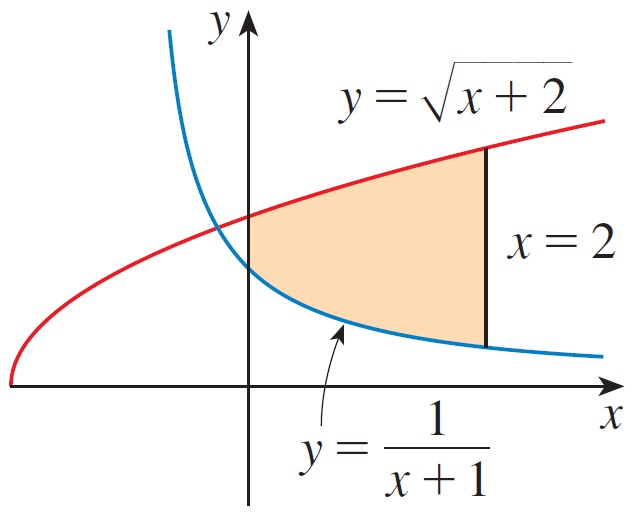
\includegraphics[scale=.3]{T-E3_1.jpg}
    
    b. 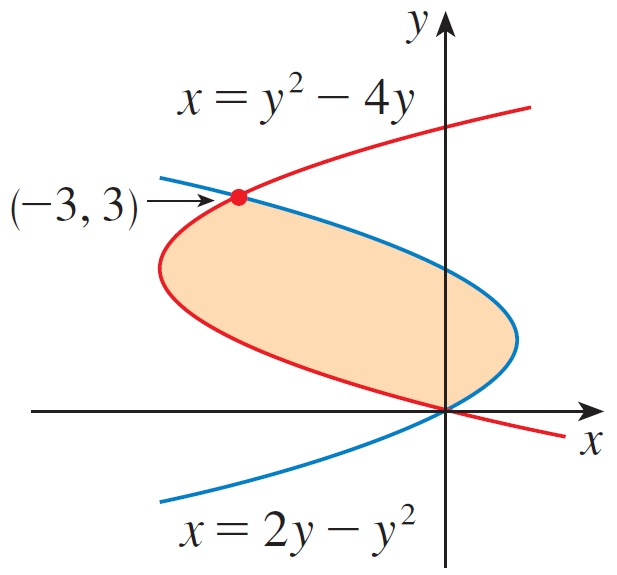
\includegraphics[scale=.3]{T-E3_2.jpg}
    \end{multicols}
%    \question Si la proporción de nacimientos de una población es $b(t)=2200e^{0.024t}$ personas por cada año y la de decesos es $d(t)=1460e^{0.018t}$ personas por cada año. Encuentra el área entre estas curvas para $0\leq t\leq 10$. ¿Qué representa el área?

%Secc. 6.5 Stewart Ej. 19
\question La densidad lineal de una varilla de 8 $m$ de longitud es $\rho(x)=\dfrac{12}{\sqrt{x+1}} \, kg/m$, donde $x$ se mide en metros desde un extremo de la varilla. Determina la densidad promedio de la varilla. 

\vskip12pt
%secc. 9.5 Stewart Review Ej. 19
\vskip10pt
\question 
\begin{enumerate}[a)]
    \item Explica por qué la función $$ f(x) = \begin{dcases} \dfrac{\pi}{20}sen \left(\dfrac{\pi x}{10}\right) & \text{si } 0 \leq x \leq 10 \\ 0 & \text{si } x < 0 \quad \text{ó }\quad  x > 10 \end{dcases}$$
    es una función de densidad de probabilidad.

    \item Encuentra $P(X<4)$
    \item Calcula la media. 
\end{enumerate}

\vskip10pt
%secc. 9.5 Stewart Review Ej. 21
\question
El tiempo gastado en la fila de espera de cierto banco se modela mediante una función de densidad exponencial con media de 8 minutos.
\begin{enumerate}[a)]
\item ¿Cuál es la probabilidad de que un cliente sea atendido en los primeros 3 minutos?
\item ¿Cuál es la probabilidad de que un cliente tenga que esperar más de 10 minutos?
%\item ¿Cuál es la mediana del tiempo de espera?
\end{enumerate}
\vskip10pt
    \question La \textit{rapidez promedio} de la molécula en un gas ideal es
    $$\bar{v}=\frac{4}{\sqrt{\pi}}\left(\frac{M}{2RT}\right)^{3/2}\mathlarger{\int_0^\infty v^3e^{-Mv^2/(2RT)}\;dv}$$
    
    donde $M$ es el peso molecular del gas, $R$ es la constante de los gases, $T$ es la temperatura y $v$ la rapidez molecular. Muestra que
    $$\bar{v}=\sqrt{\frac{8RT}{\pi M}}$$
\vskip12pt    
    \question Evalúa la siguiente integral impropia 
    $$\mathlarger{\int_0^{\infty} \frac{1}{\sqrt{x}(1-x)}\;dx}$$
    
    considerando que tiene una discontinuidad en 1. Hint: Separala en dos integrales impropias de tipo 2 y tipo 1 como sigue. 
        $$\mathlarger{\int_0^{\infty} \frac{1}{\sqrt{x}(1-x)}\;dx}=\mathlarger{\int_0^1 \frac{1}{\sqrt{x}(1-x)}\;dx}+\mathlarger{\int_1^{\infty} \frac{1}{\sqrt{x}(1-x)}\;dx}$$
\vskip12pt    
    \question Usa el teorema de comparación para determinar si la siguiente integral es convergente o divergente. 
    
    $$\mathlarger{\int_1^{\infty}\frac{2+e^{-x}}{x}\;dx}$$
  
 % \question Una alberca mide 30 pies de ancho por 50 pies de largo. La tabla muestra la profundidad h(x) del agua a intervalos de 5 pies desde un extremo de la alberca al otro. Estime el volumen del agua en la alberca por medio de la regla del trapecio con $n = 10$, aplicada a la integral
  
 % $$V=\mathlarger{\int_0^{50}30h(x)\;dx}$$
  
 % \includegraphics[scale=.3]{T-E3_3.jpg}
 \vskip10pt 
  \question 
  \begin{enumerate}[(a)]
  \item Halla las aproximaciones $T_{10}$, $M_{10}$ y $S_{10}$ para la integral $\mathlarger{\int_1^2e^{1/x}\;dx}$.
  \item Estime los errores relacionados con las aproximaciones del inciso (a).
  \item ¿Qué tan grande se tiene que elegir $n$ de modo que las aproximaciones $T_n$, $M_n$ y $S_n$ a la integral del inciso (a) sean exactas hasta 0.0001?
  \end{enumerate}
  
    \end{questions}



% Geometría para la otra carilla
\newgeometry{
	hmargin = {1.5cm, 0.5cm},
	vmargin = {0.5cm, 1cm},
	%nofoot,			% Elimina el pié
	nohead,			% Elimina el encabezado
	nomarginpar,	% Elimina las notas
	includeall,
}% \savegeometry{geometria_1}

\pagestyle{foot}    % El estilo de ésta página sólo constará de pié de página
\runningfooter{}{}{Página \thepage\ de \numpages}


%\lipsum[1-5]

% \restoregeometry
% \loadgeometry{geometria_1}


\end{document}
    \question Usando la definición de integral definida (límite de una suma de Riemann),
